% Chapter 1

\chapter{Introduction}
\label{sec:introduction}

\label{Chapter1} % For referencing the chapter elsewhere, use \ref{Chapter1} 

Ever since the creation of the first computer by Charles Babbage in the 19th century, computers
have been evolving at a rapid pace performing more and more tasks as the time passes. With this
evolution, malicious actors began to notice manners in which to subvert established systems. These
individuals, by force of belief or personal gain, have caused losses in the trillions to
organizations and individuals across the globe.

As a response to these threats, these organizations and individuals began to develop techniques and
tools to counter malicious actors. It has then, started the cat-and-mouse race between criminals
and agents of the law. One of these techniques revolves around the analysis of what software
adversaries develop to understand how they operate and the vulnerabilities they exploit to weaken
or outright topple established security systems.

This thesis presents a research about, and creation of, a method where RAG powered LLMs are
introduced onto to the malware static analysis workflow in order to increase efficiency on the
analysis.

\section{Definitions}
Here are defined all of the concepts and/or tools that are mentioned.

\subsection{Large Language Models}
Large Language Models (LLMs) are a type of multi-parameter Machine Learning (ML) algorithm designed
for natural language processing. These models that are trained on a large volume of text using a
multitude of learning techniques such as supervised and self-supervised learning.

Generative pre-trained transformers (GPTs) are the biggest and most powerful LLMs. Current models
can be adapted to certain tasks (via fine-tuning) or directed by prompt engineering
	[\cite{brown2020languagemodelsfewshotlearners}]. These models learn to predict the syntax,
semantics and ontologies found in human language, but they also pick up biases and errors from the
training data [\cite{10.1162/daed_a_01905}]. Popular examples of LLMs include:
\begin{itemize}
	\item GPT models (like GPT-4 or ChatGPT)
	\item Google's PaLM and Gemini
	\item Meta Llama series models
\end{itemize}

\subsection{Retrieval-Augmented Generation}
Retrieval-Augmented Generation (RAG)
[\cite{lewis2021retrievalaugmentedgenerationknowledgeintensivenlp}] is a technique that allows for
LLMs to query information from a specific type of datastore and use it as context for the response
it provides. This allows for adaptive learning of the models without the need of retraining
(fine-tuning). It improves the quality of LLM output as the model does not rely solely on
pre-trained knowledge but also on relevant information from the datastore.

RAG works by having the LLM to query the datastore using vector search, embeddings or keyword
matching (depending on the datastore type), feeding this data onto the LLM input and then
continuing with the normal LLM process for output generation.

\subsection{Malware}
Short for \textit{Malicious Software}, Malware is any program or code that is created for malicious
purposes like exploitation of computer systems networks or users. Often created with monetary gain
in mind, these programs activities include stealing sensitive data, damage systems, disrupt
operations or gain unauthorized access to systems or environments. Common types of malware include:
\begin{itemize}
	\item Viruses: Attach themselves to legitimate software, spreading when the software is run.
	\item Worms: Spread automatically over networks, replicating rapidly without user intervention.
	\item Trojans: Disguised as legitimate software, tricking users into installing them to enable
	      unauthorized access.
	\item Ransomware: Encrypts or locks files, demanding payment (ransom) for restoration.
	\item Spyware: Secretly collects sensitive information like passwords or browsing activity.
	\item Adware: Delivers unwanted advertisements, potentially slowing down or compromising systems.
\end{itemize}

\subsection{Malware Analysis}
As mentioned before, the software created by malicious actors needs to be evaluated and analyzed to
understand how it works, what exploits it takes advantage of and how these exploits can be patched.
As a basis, there are two types of analysis of software that can be made to understand any kind of
software. These are as follows:
\begin{itemize}
	\item \textbf{Static Analysis}: Focuses on looking at the sequences of individual instructions on the software
	      bytecode to identify the its characteristics, such as identification of the parameters in which the
	      analyzed software is built upon (e.g. Operating system it executes on, processor architecture,
	      etc), what execution paths it employs, what system calls it performs, etc. This analysis is done
	      without running the code and it requires a lot of time and effort from the analyst.
	\item \textbf{Dynamic Analysis}: Entails running the potential malicious software to gather runtime information
	      such as network calls and system call execution data which are not visible through static analysis.
	      This analysis is done by creating a special (sandbox) environment (i.e docker container and/or a virtual
	      machine) and running the software.
\end{itemize}

\subsubsection{Static vs Dynamic Analysis}
Both static and dynamic analysis have their own benefits and are important on their own right for
understanding how malware is designed and developed. While static analysis takes advantage of its
speed and safety where files do not need to be executed to be analyzed, dynamic analysis enables a
more extensive analysis which might not be visible with static analysis alone.

However, both have their limitations such as the increased computational cost and requirement of a
secure environment of dynamic analysis versus the vulnerability of static analysis to obfuscation
and encryption techniques.

% \vfill
% 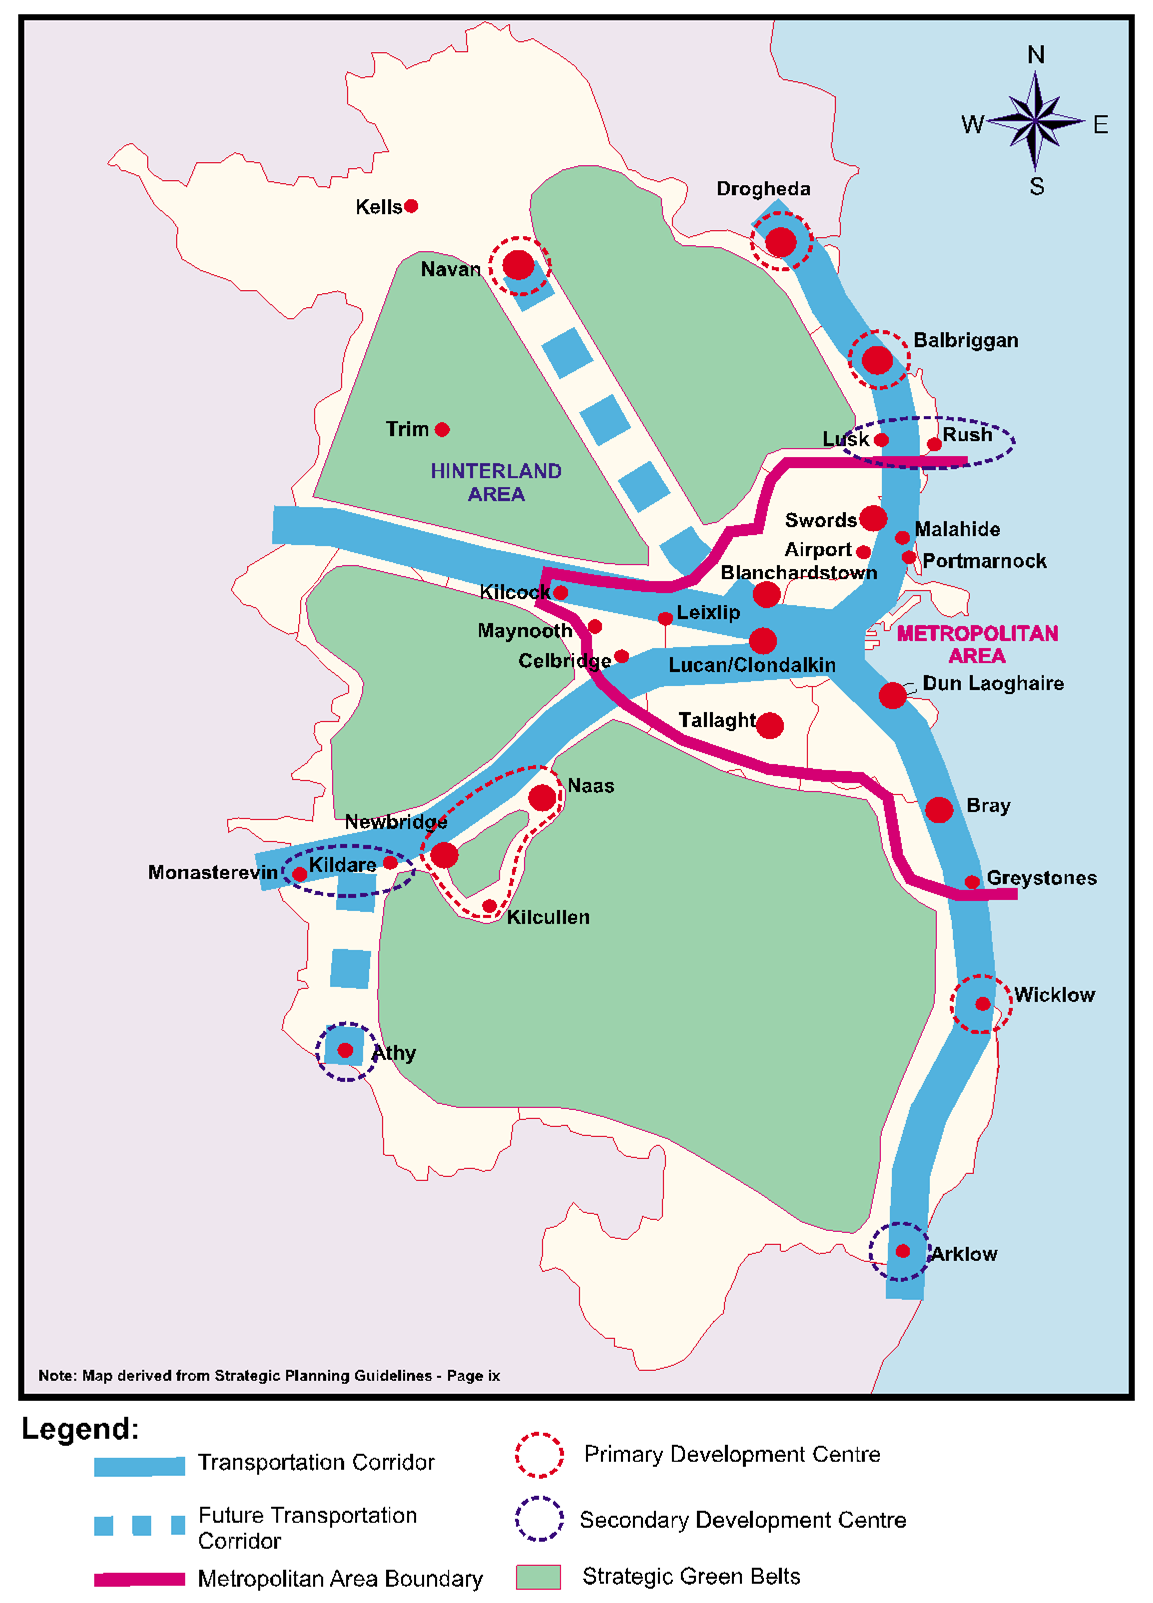
\includegraphics[width=\textwidth]{intro1.png}
% \vfill

\section{Research}

\subsection{Why?}
The reasoning behind the focus of this research is that static analysis remains to be a critical
component of malware detection and neutralization. Security analysts are often required to analyze
and process huge amounts of obfuscated data. By integrating RAG powered LLMs to this process we can
make the analysis easier by tapping onto contextual knowledge from the RAG and the analysis power
of LLMs. 

\subsection{Questions}
These are the research questions that will guide the development of this thesis.
\begin{itemize}
	\item How LLMs can be leveraged to enhance static malware analysis?
	\item How does a RAG-enhanced LLM compare to traditional static analysis techniques in terms of accuracy,
	      efficiency, and interpretability?
	\item What role does RAG play in improving LLM-driven malware classification, particularly in terms of
	      contextual relevance and justifiability of results?
\end{itemize}

\subsection{Objectives}
\begin{itemize}
	\item Develop a method for integrating LLMs with RAG to enhance static malware analysis.
	\item Evaluate the effectiveness of RAG-enhanced LLMs in identifying, explaining, and comparing malware
	      threats using static features (e.g., file structure, bytecode, API calls) against traditional
	      static malware analysis techniques in terms of accuracy, efficiency, and interpretability, while
	      identifying challenges and potential risks (e.g., adversarial manipulation and hallucination).
\end{itemize}

\subsection{hypothesis}


\section{Chapter overview}


% \section{Section Introduction}
% %always begin a section with an introduction and end it with a summery
% A thesis is built up of a series of chapters that construct a substantiated and convincing response
% to the research question(s). Typically, a thesis contains the following chapters: an introduction;
% a literature review; a description of methodology; a report and discussion of results; and a
% conclusion. A thesis may have five to eight chapters depending on the nature of the study, the
% required word count and the requirements of the degree.

% \subsection{About the Introduction Chapter}
% An introduction is crucial to setting the tone of your thesis – it is the first impression you’ll
% make on your readers (assessors). Briefly, it presents the purpose, context and scope of your
% research. Likewise, a conclusion is just as crucial – it is the lasting impression you’ll make on
% your readers (assessors). Not only does it give a summary of your thesis, but should provide a
% clear, convincing answer to your research question(s).
% \subsection{Subsection header 2}
% After introducing your work, you should list your research questions, hypothesis, and objectives.

% Always keep in mind the meaning of the word ``\textit{Thesis}''. That is: a thesis is a statement
% or theory that is put forward as a premise to be maintained or proved. A Hypo\textit{thesis} then,
% is a sub-thesis, or a smaller part of the overarching thesis.

% All of your research questions must aim to prove or disprove your thesis.. and thus your
% hypotheses.

% See more here: \url{https://www.statconsul.com/research-questions.php}
% \subsection{Subsection header 3}
% The last thing you do in an Introduction Chapter is to outline the contents of your thesis, i.e., a
% review of then literature is provided in Chapter \ref{sec:LitReview}, starting with... etc...
% Chapter \ref{sec:Method} provides a description of the method... etc...

% \section{More about the Introduction chapter}
% The introduction allows you to orient the reader to your research project and preview the
% organisation of your thesis. In the introduction, state what the topic is about, explain why it
% needs to be further researched and introduce your research question(s) or hypothesis.

% Whilst patterns of organisation in introductions vary, there are some common features that will
% help you to achieve an informative and engaging introduction. Let’s identify these features:

% \begin{itemize}
% 	\item Introduce the topic
% 	\item Define key terms and concepts
% 	\item Give background and context for the topic (this may include a brief literature review)
% 	\item Review and evaluate the current state of knowledge in the topic (this may include a brief
% 	      literature review)
% 	\item Identify any gaps, shortcomings and problems in the research to date
% 	\item Introduce your research question(s) or hypothesis
% 	\item Briefly describe your methodology and/or theoretical approach
% 	\item Explain the aim of your research and what contribution it will make to the topic
% 	\item Give an overview of the chapter outline of the thesis.
% \end{itemize}

% It’s important to note that, depending on your field of study and the faculty requirements of your
% thesis, not all of these features will be relevant. Also, these features may occur in varied
% orders.

% Most people write many drafts of their introduction. It can be useful to write one early in the
% research process to clarify your thinking. You will need to write a version for your confirmation
% proposal and other milestones. As your research progresses and your ideas develop, you will need to
% revise it. When the final draft of chapters is complete, check the introduction once more to make
% sure that it accurately reflects what you have actually done.
